% QUESTAO
Usando a Lei dos Senos no triângulo abaixo, determine o valor do lado $x$:
(Considere $\text{sen}\,30^\circ = \frac{1}{2}$ e $\text{sen}\,45^\circ = \frac{\sqrt{2}}{2}$)

\parbox{0.3\linewidth}{

% ALTERNATIVAS
$10\sqrt{2}$
$5\sqrt{2}$
$10$
$20$
$5$

}\parbox{0.7\linewidth}{
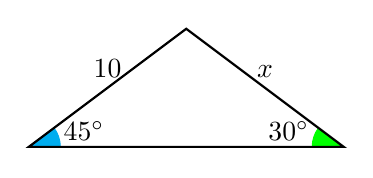
\begin{tikzpicture}[scale=1]
	\draw[cyan, fill] (0,0) -- (0.4,0) arc (0:36.87:0.4) -- cycle;
	\draw[green, fill] (4,0) -- (3.6,0) arc (0:-36:-0.4) -- cycle;
	\draw[thick] (0,0) -- (4,0) -- (2,1.5) node[midway, above] {$x$} -- node[midway, above] {$10$} cycle;
	\node at (0.7,0.2) {$45^\circ$};
	\node at (3.3,0.2) {$30^\circ$};
\end{tikzpicture}
}


